\documentclass[crop=false,10pt,ngerman]{standalone}
\usepackage{standard}
\begin{document}
  \section{Implementierung} % (fold)
  \label{sec:implementierung}

    \subsection{Repräsentation des Berechnungsgebietes} % (fold)
    \label{sub:repräsentation_des_berechnungsgebietes}
      Es handle sich bei $[\domain]\define\roundBrackets{\domain,\dirichletBoundary,\neumannBoundary,ν}$ wieder um ein Berechnungsgebiet.
      Die Implementierung einer Finite-Elemente-Methode verlangt die Diskretisierung von $[\domain]$, wie es in Abschnitt \ref{ssub:discretization-domain} beschrieben wurde.
      Es sei $(V,E,\mathscr{T})$ eine Triangulierung von $[\domain]$.
      Die Implementierung der Basisstruktur für die Triangulierung des Berechnungsgebietes sei durch den folgenden Quelltext gegeben.

      \inputCodeBlock[title=domain\_base]{code/domain_base.cc}
      Die Basisstruktur wird als \code{Domain\_base} im Namespace \code{Fem} konstruiert.
      In ihr werden die Strukturen \code{Edge} und \code{Primitive} für die Beschreibung der Kanten und Dreiecke deklariert.
      Die verschiedenen Konstruktoren und Zuweisungsoperatoren der Sprache C++ werden explizit durch den Compiler erzeugt.
      Der Destruktor wurde mit \code{virtual} gekennzeichnet, wie es für polymorphe Basisklassen angebracht ist \cite[S.~40~ff]{Meyers2008}.

      \inputCodeBlock[title=edge]{code/edge.cc}

      \inputCodeBlock[title=primitive]{code/primitive.cc}

      \inputCodeBlock[title=domain]{code/domain.cc}

      \inputCodeBlock[title=domain implementation]{code/domain_implementation.cc}

      \inputCodeBlock[title=subdivide]{code/domain_implementation_subdivide.cc}

      \begin{center}
        \noindent
        \begin{minipage}[b]{0.32\textwidth}
          \begin{tcolorbox}[titlerule=0.1pt,boxrule=0.5pt,arc=5pt,title={Zeile 1-13}]
            \lstinputlisting[style=standard,firstline=1,lastline=13]{code/model-test.txt}
          \end{tcolorbox}
        \end{minipage}
        \hfill
        \begin{minipage}[b]{0.32\textwidth}
          \begin{tcolorbox}[titlerule=0.1pt,boxrule=0.5pt,arc=5pt,title={Zeile 14-26}]
            \lstinputlisting[style=standard,firstline=14,lastline=26]{code/model-test.txt}
          \end{tcolorbox}
        \end{minipage}
        \hfill
        \begin{minipage}[b]{0.32\textwidth}
          \begin{tcolorbox}[titlerule=0.1pt,boxrule=0.5pt,arc=5pt,title={Zeile 27-39}]
            \lstinputlisting[style=standard,firstline=27,lastline=39]{code/model-test.txt}
          \end{tcolorbox}
        \end{minipage}
      \end{center}

      \begin{figure}[h]
        \begin{subfigure}[b]{0.24\textwidth}
          \center
          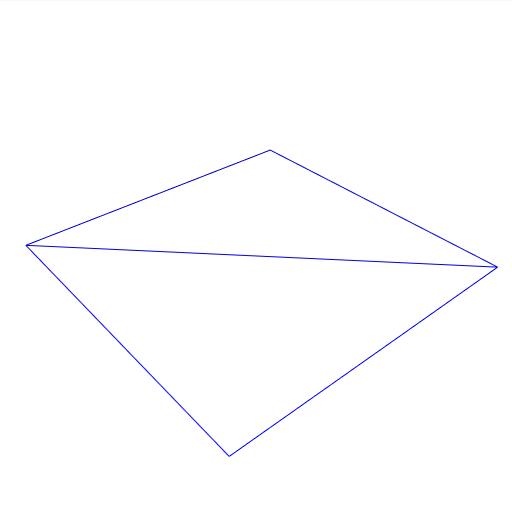
\includegraphics[trim={0 0 0 2cm},clip,width=0.95\textwidth]{images/model-quad-0.png}
          \caption{Quad}
        \end{subfigure}
        \begin{subfigure}[b]{0.24\textwidth}
          \center
          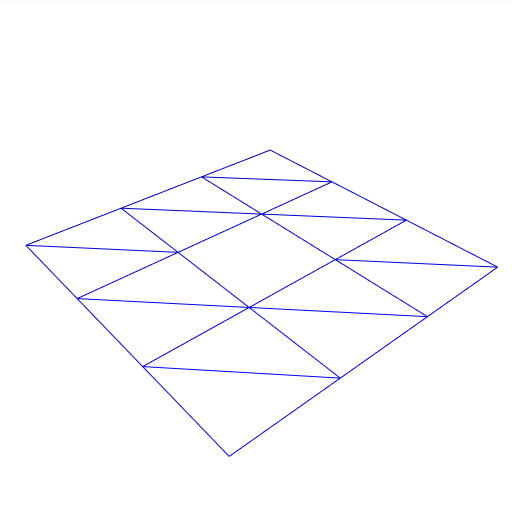
\includegraphics[trim={0 0 0 2cm},clip,width=0.95\textwidth]{images/model-ring-0.png}
          \caption{Ring}
        \end{subfigure}
        \begin{subfigure}[b]{0.24\textwidth}
          \center
          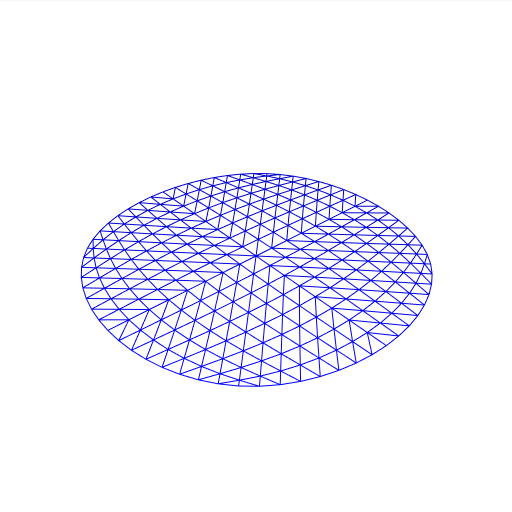
\includegraphics[trim={0 0 0 2cm},clip,width=0.95\textwidth]{images/model-circle-0.png}
          \caption{Curved}
        \end{subfigure}
        \begin{subfigure}[b]{0.24\textwidth}
          \center
          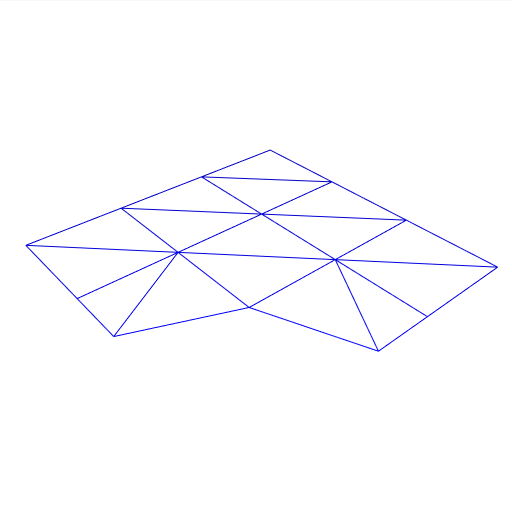
\includegraphics[trim={0 0 0 2cm},clip,width=0.95\textwidth]{images/model-test-0.png}
          \caption{Test}
        \end{subfigure}
      \end{figure}

      \begin{figure}[h]
        \begin{subfigure}[b]{0.24\textwidth}
          \center
          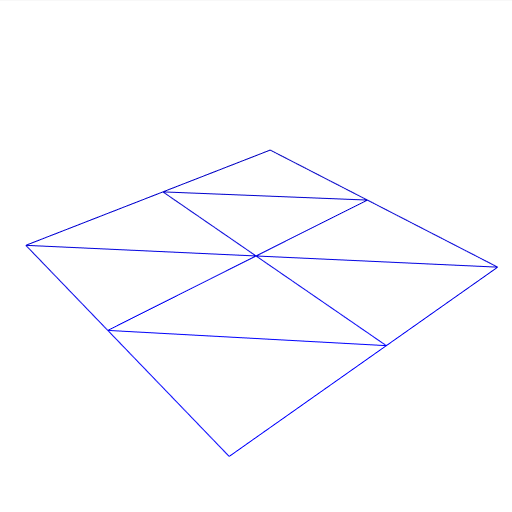
\includegraphics[trim={0 0 0 2cm},clip,width=0.95\textwidth]{images/model-quad-1.png}
          \caption{Quad}
        \end{subfigure}
        \begin{subfigure}[b]{0.24\textwidth}
          \center
          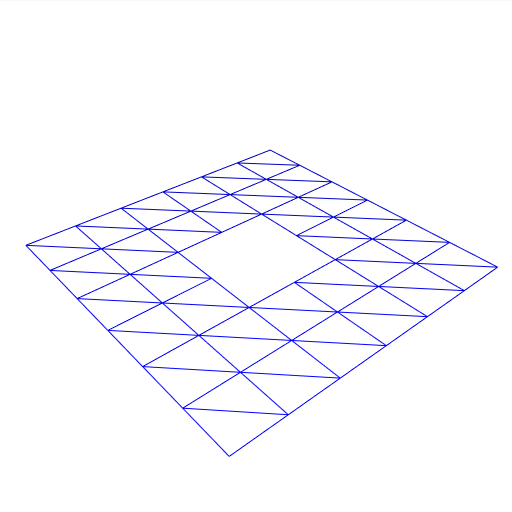
\includegraphics[trim={0 0 0 2cm},clip,width=0.95\textwidth]{images/model-ring-1.png}
          \caption{Ring}
        \end{subfigure}
        \begin{subfigure}[b]{0.24\textwidth}
          \center
          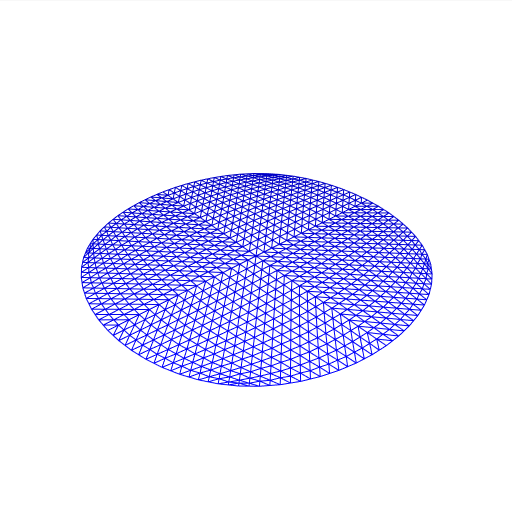
\includegraphics[trim={0 0 0 2cm},clip,width=0.95\textwidth]{images/model-circle-1.png}
          \caption{Curved}
        \end{subfigure}
        \begin{subfigure}[b]{0.24\textwidth}
          \center
          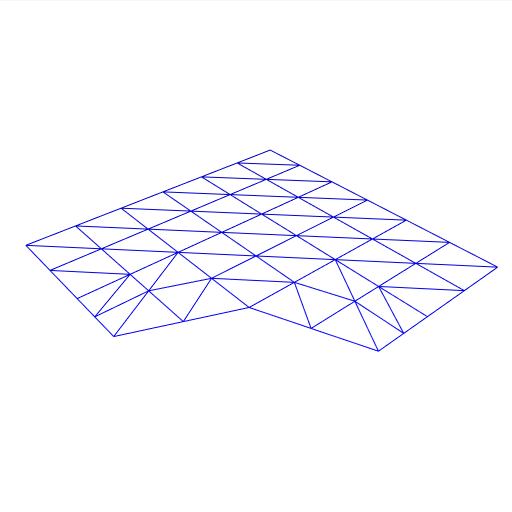
\includegraphics[trim={0 0 0 2cm},clip,width=0.95\textwidth]{images/model-test-1.png}
          \caption{Test}
        \end{subfigure}
      \end{figure}

      Das Gebiet $\Omega$ kann nur in Dreiecke unterteilt werden.
      Wir trennen Eckpunkte und Primitive, wie im OBJ-Dateiformat.
      Weiterhin werden Kanten für Neumann- und Dirichlet-Randbedingungen extra aufgeführt.
      Dies ist möglich, da die Randbedingungen unabhängig von den Primitiven betrachtet werden können.
      Die Primitive müssen demnach nicht auf die Ränder verweisen.
      \cite{Alberty1998}
    % subsection repräsentation_des_berechnungsgebietes (end)

    \subsection{Konstruktion der Mass und Stiffness Matrix} % (fold)
    \label{sub:konstruktion_der_mass_und_stiffness_matrix}

      \inputCodeBlock[title=Wave system]{code/cpu_wave_system.cc}

      \inputCodeBlock[title = GPU Wave system]{code/gpu_wave_system.cc}

      \inputCodeBlock[title = System construction]{code/cpu_wave_system_constructor.cc}

      \inputCodeBlock[title = System construction]{code/gpu_wave_system_constructor.cc}

      \inputCodeBlock[title = System construction]{code/gpu_wave_system_destructor.cc}

      \inputCodeBlock[title = System construction]{code/gpu_wave_system_accessors.cc}

      \inputCodeBlock[title = CPU Wave System advance]{code/cpu_wave_system_advance.cc}

      \inputCodeBlock[title = GPU Wave System advance]{code/gpu_wave_system_advance.cc}

      \inputCodeBlock[title = Conjugate Gradient]{code/cpu_conjugate_gradient.cc}
      \inputCodeBlock[title = GPU Kernel]{code/gpu_wave_system_kernel.cc}

    % subsection konstruktion_der_mass_und_stiffness_matrix (end)

    \subsection{Konstruktion des linearen Gleichungssystems} % (fold)
    \label{sub:konstruktion_des_linearen_gleichungssystems}

    % subsection konstruktion_des_linearen_gleichungssystems (end)

    \subsection{Lösen des Gleichungssystems} % (fold)
    \label{sub:lösen_des_gleichungssystems}

    % subsection lösen_des_gleichungssystems (end)

    \subsection{Randbedingungen} % (fold)
    \label{sub:randbedingungen}

    % subsection randbedingungen (end)

    \subsection{Visualisierung} % (fold)
    \label{sub:visualisierung}

    % subsection visualisierung (end)
  % section implementierung (end)
\end{document}